\documentclass[12pt,titlepage]{report}
\usepackage{graphicx}
\usepackage{hyperref}
\usepackage{subcaption} 
\hypersetup{colorlinks=true}
\begin{document}
\title{\Huge{Argus} 
\\  \large\emph{User Manual}}
\author{Matthew Crispin Scicluna}
\maketitle
\pagebreak
\tableofcontents
\chapter{Introduction}
\section{What is Argus?}
Argus is a computer program written in the programming language R. It was written by Matthew Scicluna from June 2013 to August 2014. Argus' main purpose is to assist Biologists and Pychologists in the study of animal behavior. It achieves this by converting the raw output from an existing video tracking program into meaningful statistics that can be interpreted by researchers. This raw ouput consists of the x-y coordinates of the fish as well as the arena dimensions. Often they are unscaled and very difficult to read, let alone analyze meaningfully! Argus aims to translate this raw data into easy to understand statistical output that can be used to strengthen the researchers findings. Argus also has an added flexibility due to its status as freely available shareware. Argus can be made to run any custom script the user desires, and can interpret data from any tracking system. It is due to this flexibility that Argus can be made to perform many custom applications that would be too specialized for other comercially available software to perform. In later chapters several such applications will be discussed.

Before you can do any analysis with Argus you must first choose a video tracking program to get the raw output from. In the next chapter we will discuss one such tracking program.


\section{What is theRealFishTracker?}
Argus was originally made to exclusively utilize a previously created program called theRealFishTracker, built by James McCrae in 2011. A good description of the program and its download information can be found at \url{http://www.dgp.toronto.edu/~mccrae/projects/FishTracker/}. The program converts a video file into a text document. The output can be analyzed using theRealFishTracker itself, but the programs own analysis is suboptimal for the kinds of large scale data sets expected in modern psychological and biological research.The raw text file can instead be read into Argus.
 
\section{Other Video Tracking Systems}
Argus comes with scripts to analyze the output from theRealFishTracker and Ethovision. It can be made to analyze any other video tracking system's raw output. The user must write a script that converts the raw output into a dataframe that can be used within Argus, however. Such scripts will be released in the future based on the demand for them.


\begin{figure}[ht!]
\centering
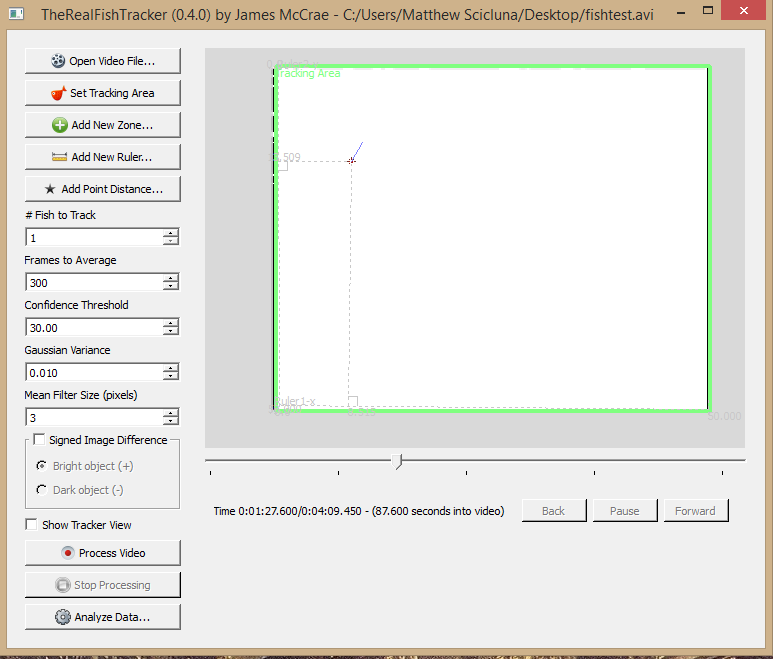
\includegraphics[width=120mm]{image12.png}
\caption{RealFishTracker Interface}
\label{overflow}
\centering
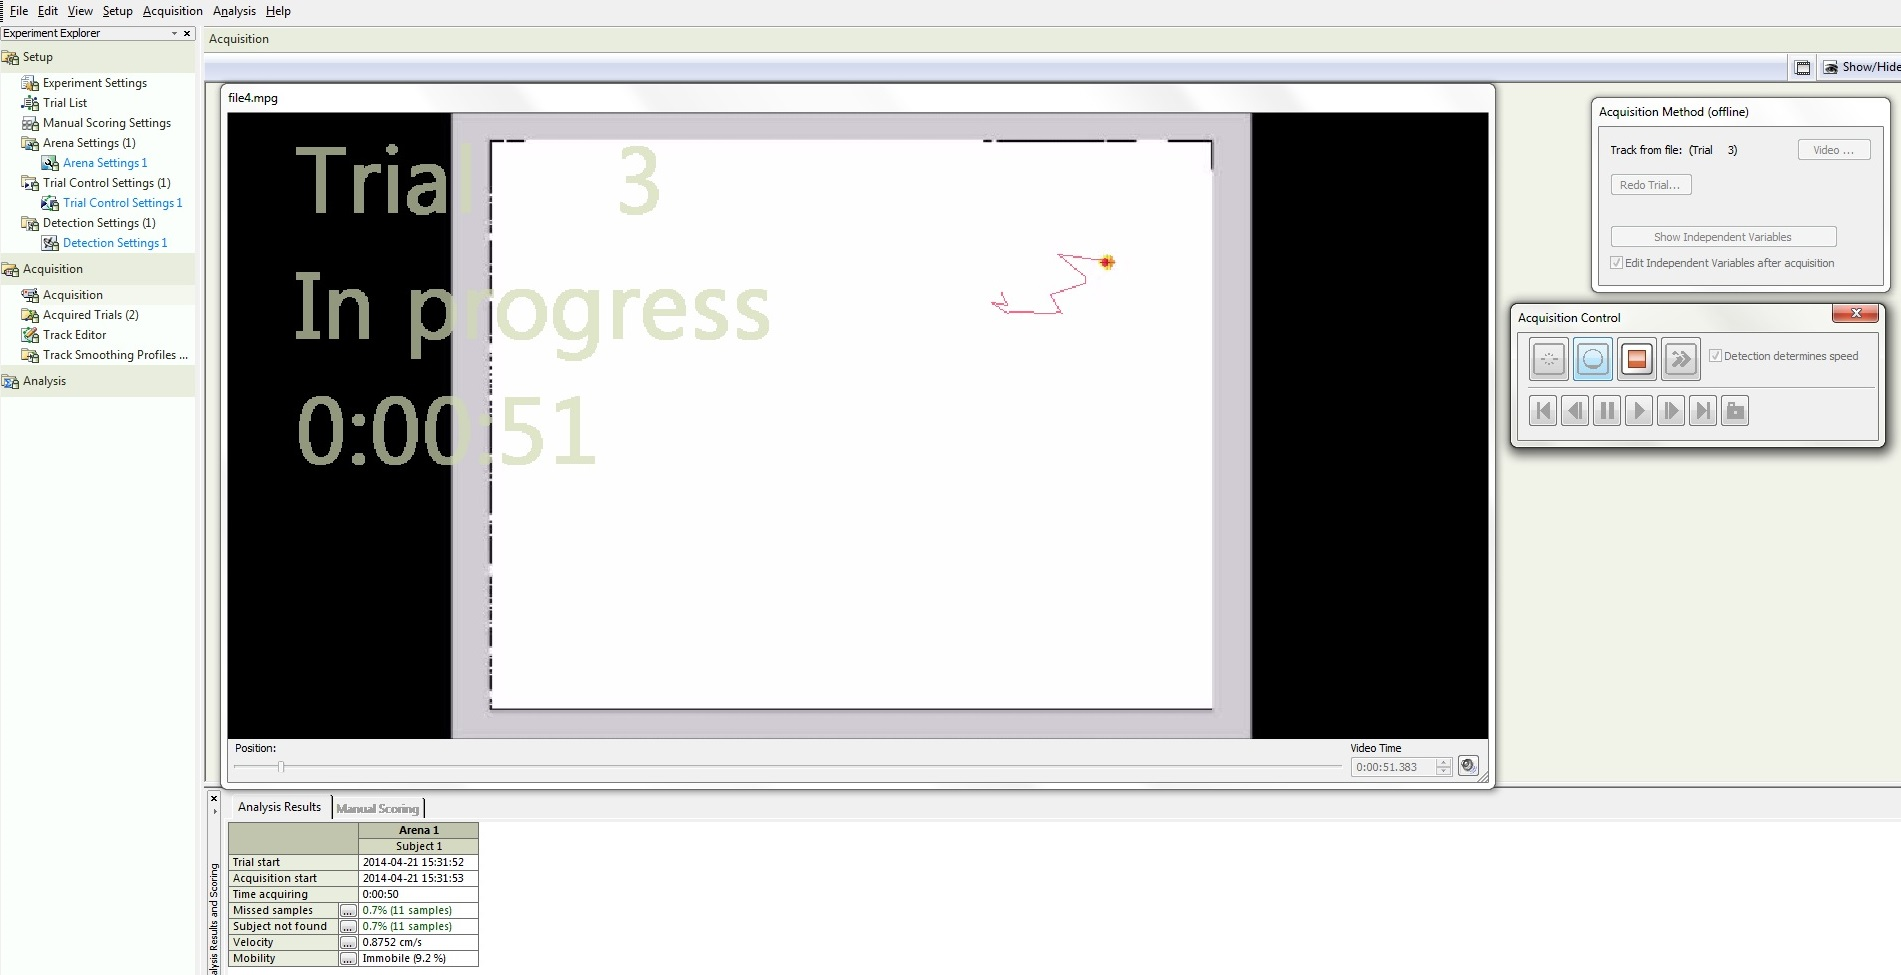
\includegraphics[width=120mm]{image14.png}
\caption{Ethovision Interface}
\label{overflow}
\end{figure}

\chapter{Startup}
\section{Installing Argus}
In order to install Argus, you will have to install R and the packages: \texttt{ RGtk2Extras}, \texttt{gWidgets}, \texttt{RGtk2}, \texttt{xlsxjars} and \texttt{rjava}. The package \texttt{rjava} additionally requires that you have java installed on the computer. More information about R and any of its packages can be found online at \url{http://cran.r-project.org/}.
 Argus consists of several program files, the core ones being: the text documents \emph{fish analyzer program}, \emph{multi case fish analyzer program} and \emph{load GUI} and the R file \emph{GUI frontend}. There should also be additional files which are used for converting the output for tracking software for Argus. Any customly written program files would be put here as well. The aforementioned files should be in a folder called scripts which should be inside of a folder called Argus. Also inside the Argus folder is to be another folder where the text files from theRealFishTracker or any other tracking softwares are to be stored. This new folder will hold the files to be analyzed by Argus.
To begin running Argus, place the text file output from theRealFishTracker, or whatever video tracking software you are using into the folder mentioned above. This program can process as many output files from tracking softwares as you want, and will analyze them all simulteneously. \\
\paragraph{A Note About What Not to Do}
Be mindful of the similarities between files that you put into the folder in this program. If you desire a uniform number of time bins, then you should not put files with significantly varying times, unless you strickly specify the number and time of each bin in such a way that their product is less than the time elapsed in the shortest time bin (more on this in chapter 3). Also note you shouldn't simulteneously process output files from different tracking softwares.\\

\section{Running Argus}
Upon installation, to begin using Argus, one must open the R terminal (by clicking on the R icon). Load the R script \texttt{loader}. This script should be found in the argus folder. Once loaded, you should see a line of code that looks like this:

\begin{verbatim}
program_directory<-"C:\\Users\\Matthew Scicluna\\Desktop\\Argus"
\end{verbatim}

Modify the aformentioned line of code with the location of the Argus folder on your computer and run the two commands on the script in order to load Argus. This second part can be done on a PC by pressing the F5 key twice. Once loaded, The GUI will appear and allow the user to specify what actions the program is to do with the files. 

\section{Navigating the GUI}
The GUI of Argus is split into 2 windows. The main window has 3 sections: a menu bar, left panel with 3 tabs and right panel. The second window displays the command history, so the user has a history of all of their actions. The menu bar contains 3 icons: open, help and close. The Open button allows the user to select the files to be run with the program. pressing the help button opens up the help window, which provides information about the functions of Argus. Pressing the close button terminates the program.

\subsection{Loading the Output Files}
The first thing the user should do is load the directory where the theRealFishTracker output files were placed. This is done by pressing the folder icon on the menu bar on the top left side of the GUI. Selecting the folder with the trials will cause the program to set its default directory there. Once the folder is selected the user must select the number of bins, times of bins, or a combination of the two. This will be described in greater detail in the next section. The user must also specify the number of fish they used in their trial(s). Once this is done the user can select functions and parameters for the functions.

\subsection{Select Conditions}
It is here where you can specify the tracking software you are using, the number of bins you want the program to make, the time of each bin (in seconds), the number of fish being tracked in your files and the number of factors you want to appear in the Excel output, for which you would select at a later time. To specify the conditions you want, just enter the appropriate numbers in the appropriate fields, bearing in mind the units of measurement when applicable. The tracking systems which Argus can utilize currently are Noldus Ethovision and theRealFishTracker. To specify which tracker you are using, you would enter either ETH or RFT, respectively. Argus allows for its users to write additional scripts so it can manage new software programs, and the user can go into the source code and simply add a new 3 letter indicator to be able to extend Argus' functionality to whichever program they desire to use. Once this is complete and you have selected all of the commands, parameters and options, you can press the run button to advance to the next screen. This will be covered in more detail in a later chapter. 
\subsection{Advanced Options}
There are two additional checkboxes in this panel, one called 'Advanced Behavioral Detials' and another called 'Frame-by-Frame Features'. By pressing the 'Frame-by-Frame Features', one can get an excel printout of every frame of every bin of every trial recorded along with all of the frame by frame features such as instantaneous speed at each timeframe and the turn angle at each timeframe. This output can be fed into external machine learning algorithms to try to classify and detect particular behaviors.
The 'Advanced Behavioral Details' gives the user an additional Excel output file. This file contains the start time, end time and total duration of each behavior detected by the program, and can be of assistance for any researcher who wants to compare the accuracy of the functions detection abilities with previously scored behavioral data. The start and end times can also be used to retrieve the frames from the advanced output where the desired behavior occurred during for use as a training set in a machine learning algorithm.

\begin{figure}[ht!]
\centering
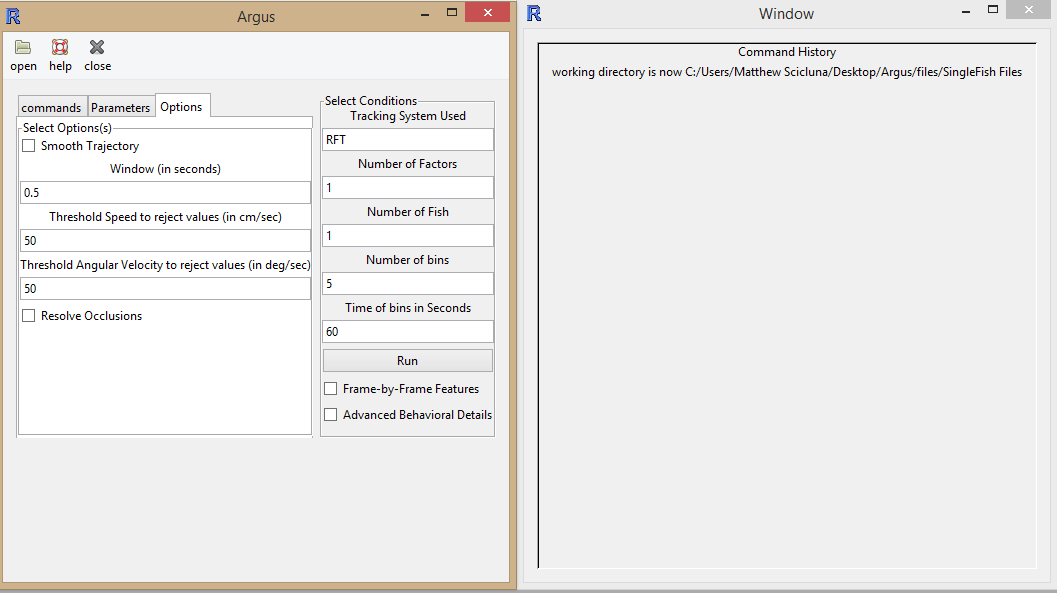
\includegraphics[width=150mm]{image11.png}
\caption{Argus GUI}
\label{overflow}
\end{figure}

\chapter{Functions and Parameters}
Now that you have specified the directory of the folder, the number of fish and kinds of time bins you want; you are ready to specify the kind of information you want Argus to extract from the raw text files generated from the video tracking program. The left panel in the GUI contains all the functions available to call, as well as the parameters for them, in a seperate tab. In the GUI, functions are called Commands. We should clarify what we mean by functions and parameters, so here is a definition of both.
\paragraph{What is a Function?}
A function is basically a set of commands that may or may not require user input to produce useful statistics for the user. Essentially we are asking the computer to interpret the data in some specific way. An example of a function would be the first function I wrote for this program, which is the speed function. This function takes no parameters but will tell the user how fast the fish travelled in during the duration of the trail, measured in cm/sec.
\paragraph{What is a Parameter?}
A parameter is a value that is associated with a function. Changing the value of the parameter may change the value of the output statistic of the function. An example of this is the Thigmotaxis function. The thigmotaxis function produces a statistic which is the average distance the fish was from some point in the fish tank. This point is specified by an x and y coordinate, which are the functions 2 parameters. It can be seen that changing the parameter (and thus specifying a new point) will affect the statistic, as it is now measuring the average distance of a fish to a \emph{different} point. 
\section{Two Kinds of Variables}
Argus has two different kinds of variables it can measure: Trajectory variables and behavioral variables. Trajectory variables are calculated using widely accepted formulas that do not differ much among different tracking programs. This is not the case for behavioral variables, which do not have any particularly widespread detection criterion. Argus handles analyzing these kinds of variables by giving the user many possible parameters to work with in defining the behavior. The user is also free to use the Advanced output generated by Argus in programs that utilize supervised and unsupervised learning techniques. It should be apparent to the reader which variables measured using commands from Argus fall into which variable category.

\section{Functions for Single Fish Trials}
Functions in Argus only either work for trials with tracking of a single fish, or with trials with tracking of multiple fish. These are the functions that work only for analyzing trials where one fish was tracked. These functions will not work if you use them in trials where multiple fish were tracked at once. To select a function, press the box on the left of the function's name. Here is a complete list of all the functions available in Argus, along with the parameters for each that the user can specify.

\subsection{SPEED}
Calculates speed, acceleration, distance travelled and fastest speed of the fish during each time bin.
\subsection{THIGMOTAXIS}
Average distance from fish to a point in the fishtank specfied by the parameters \texttt{X coord} and \texttt{Y coord}. 
\subsection{TIMESPENT}
Calculates the time fish spent accelerating, changing direction, staying still, and moving at particular speeds during each time bin.
\subsection{DISTANCE FROM SIDES}
Calculates the average distance the fish was to each side and to the top and bottom of the fish tank during the duration of each time bin.
\subsection{TIME AT OUTER PERCENT}
Calculates the time the fish spent in the periphery of the fishtank. The periphery is specified by the parameter \texttt{Percentage}, which represents the inner percentile of the fishtank for which this function calculates the time the fish was away from.
\subsection{FREEZING}
Number of times fish was detected freezing. The parameters are: 
\begin{itemize}
\item \texttt{Percent of Tank}: The outer periphery the fish must be in for freezing to be considered happening and \item \texttt{Number of Seconds}: The number of seconds fish performs freezing activity for program to consider it freezing.
\end{itemize}
\subsection{FLOATING}
Number of times fish was detected floating. The parameters are: 
\begin{itemize}
\item \texttt{Number of Seconds}: the number of seconds fish performs floating activity for floating to be considered to have happened 
\item \texttt{Percent of Tank}: the outer percentile of tank fish need to be \emph{in} for duration of behavior for it to be considered for floating.                                                      
\end{itemize}
\subsection{LEAPING}
Number of times fish was detected leaping. Parameters are: 
\begin{itemize}
\item \texttt{Speed Exceeded}: the minimum speed fish must maintain during leaping behavior for program to recognize behavior
\item \texttt{Number of Seconds}: the number of seconds fish performs leaping activity for program to consider it leaping.
\end{itemize}
\subsection{ERRATIC}
Number of times fish was detected having erratic behavior. Parameters are: 
\begin{itemize}
\item \texttt{Percent of Tank}: the outer percentile of tank fish needs to be in for behavior to be considered erratic \item \texttt{Speed Exceeded}: minimum speed fish must maintain during erratic behavior for program to recognize behavior
\item \texttt{Number of Seconds}: number of seconds fish performs erratic activity for program to consider it erratic.
\item \texttt{Number of Turns}: minimum number of turns the fish must perform during the erratic activity for program to consider it erratic.
\end{itemize}
\subsection{THRASHING}
Number of times fish was detected thrashing. Parameters are: 
\begin{itemize}
\item \texttt{Percent of Tank}: percentile of tank fish must be swimming outside of for behavior to be considered thrashing. \item \texttt{Number of Seconds}: number of seconds fish performs thrashing activity for program to recognize behavior.
\item \texttt{Number of Turns}: minimum number of turns the fish must perform during the thrashing activity for program to consider it thrashing.
\end{itemize}
\subsection{CUSTOM}
Number of times fish was detected performing a custom behavior with every possible parameter setting. Parameters are: 
\begin{itemize}
\item \texttt{Within Percent of Tank}: the outer percentile of tank fish needs to be in for behavior to be considered erratic
\item \texttt{Outside Percent of Tank}: percentile of tank fish must be swimming outside of for behavior to be considered.
 \item \texttt{Number of Seconds}: number of seconds fish performs thrashing activity for program to recognize behavior.
\item \texttt{Number of Turns}: minimum number of turns the fish must perform during bouts of the behavior for program to recognize the behavior.
\texttt{Minimum Speed}: minimum speed fish must maintain during bouts of its behavior for program to recognize behavior.
\texttt{Maximum Speed}: maximum speed fish is allowed to have during  bouts of its behavior for program to recognize the behavior.
\end{itemize}

\section{Functions for Multiple Fish Trials}
If you have trials where multiple fish are being tracked at once, you can use all the above functions, but in addition can also use the following functions.
\subsection{IID}
\emph{Inter Individual Distance} The average distance from each fish to each of the other fish. This function will produce this statistic for each fish tracked. So if there are 3 fish in your trial, this function will generate the average of the average distances from fish 1 and 2; and fish 1 and 3. These values will appear in the printout in adjacent rows.
\subsection{VIID}
\emph{Variance of Inter Individual Distance} The variance between the average distance between each fish and each other fish. Also produces a value for each fish being tracked in each trial.
\subsection{NND}
\emph{Nearest Neighbour Distance} The distance from each fish to its "nearest neighbour" --- the fish that was physically closest to it during the duration of each time bin. Produces a statistic for each fish.
\ 
\chapter{Options}
The third tab in the left panel of the main window allows the user to select additional options for processing the behavioral trials. These options are:
\section{Smooth Trajectory}
The program can smooth the trajectory of the fish using a weighted moving average. This can help to remove the stochastic noise frame to frame. The amount of seconds to average over is a parameter that can be set. An additional parameter that can be set is the option to ignore data points that would imply movement of a fish above so threshold value. These data points would be ignored during the averaging process during the smoothing.

\section{Resolve Occlusions}
In addition to smoothing the trajectory, Argus also has a built in method that can resolve occlusions. Argus does this by making the assumption that two fish crossing each other will not change direction considerably relative to where they were previously. Based on this principle it will reconstruct each occluding fishes trajectory to minimize the turn angle of each fish at the time of the occlusion, swapping trajectories at that point if necessary. In this sense the program will select the trajectory with the minimum turn angle. This seems to be the standard method to resolve occlusions in the literature.

\chapter{Additional Capabilities}
A strength of Argus is its internal representation of the behavioral data which is accessible through R’s command line after Argus has executed (the command line is NOT contained in the GUI of Argus).

\section{Indexing Internal Data Structures}
To access the advanced output for any fish in any time bin during any of the recorded trials enter the following into the command line:
\begin{verbatim}
>db[[trial #]][[bin #]][[fish #]]
\end{verbatim}
Or for trials with just one fish:
\begin{verbatim}
>db[[trial #]][[bin #]]
\end{verbatim}
Because of this, one can continue to query and analyze results from Argus without leaving R’s interactive environment, allowing the researcher to be able to perform a battery of possible analysis within R. One can of course also use the excel spreadsheet output from Argus for analysis using programs such as SPSS, SAS etc...
Argus was built to read files from theRealFishTracker, but scripts can be easily written that would allow it to read the output of files from other programs available like Ethovision. This data can analyzed with Argus’ built in functions and exported via Excel spreadsheets or analyzed within Argus itself using its internal storage to querying its extracted frame-by-frame features.
The data from Argus’ functions are also available from the command line after Argus has finished executing. They can be retrieved by   entering the following into the command line:
\begin{verbatim}
>functions[[index number of function]]
\end{verbatim}
*the index number of a function is a unique number that corresponds to the output table of a particular function. This number is different if you are using one fish versus multiple fish. You will have to look the number up in a table.
If you wanted to find the total distance travelled by the fish (assuming you ran Argus and selected the speed function to execute) you would input into the command line:
\begin{verbatim}
>functions[[1]]
\end{verbatim}
Since 1 is the number that refers to the total distance travelled.
\section{Neural Network Behavior Classifier}
Argus has several scripts written to take information from the db internal data structure (described previously in section 5.1) and train a neural network for classification of behaviors.
subsection{Classification of Behavioral Variables}
Recall in section 3.1 a distinction was made between trajectory variables and behavioral variables. There are formulas that allow any researcher to compute trajectory variable values analytically uncontroversially. The computation of behavioral variables is a much more challenging task as there is no accepted formula to compute them. There is also disagreement in the literature as to the features that classify these behaviors. The result of this is that the classification of behaviors can vary by researcher and by experiment. Behavior classifications made within an experiment can also vary observer to observer Reliability measures are often employed to control for the subjectivity inherent in these kinds of variables.

Recently machine learning algorithms have been utilized to deal with classification problems like behavior recognition to some success. Argus has an internal data structure that is organized to allow for researchers to run these kinds of algorithms on the results of their experiments. In the next section a neural network algorithm will be described that can be trained to predict animal behavior using several scripts written to interact with the internal data bases in Argus. These scripts can be modified to create more complex classifiers with higher accuracy.

\subsection{Preparation}
To begin training a behavior classifier, one needs to have their files seperated appropriately into the 4 subfolders in the \texttt{ML} folder in the \texttt{files} folder in Argus. Two of these folders hold the log files and two hold the raw output from Argus.
\\
paragraph{Log files} The log files refer to the output file from Observer. This files contains the a description of which behaviors are occuring at each time frame. These behaviors would have been manually recorded. The raw output from the videos pertaining to these log files will be in a different subfolder. One should be careful not to break this correspondance or the training algorithm will fail as it will attempt to match labels from the log files to the wrong videos! It is for this reason that one should also make sure the cutoff times are accurate, or the entire video will have instances of the behavior incorrectly labeled at every time point. The log files will go into one of two folders depending on if it will be in the training set or the test set.
\\
paragraph{Training Set vs. Test Set} The training set consists of the data the program directly trains on. The test set consists of the data the program attempts to make predictions about. The training set of files will need to be coded in observer manually beforehand in order for the labels to be utilized by the learning algoritm in Argus. The test set will need to be coded in observer as well if the researcher wants to check the accuracy of the classifier.

\subsection{Bypass the GUI}
The first script that should be executed is callled \texttt{Bypass GUI}. This script will run Argus automatically without the user interface. This is done to avoid the loading time of the GUI and to avoid having to manually input the cutoff times (the cutoff times can be added directly to the script). Running this script will create the \texttt{db} object for which the classifier learns the features of. One should note that this script can be executed \emph{anytime} the user wants to avoid loading the Argus GUI, and likewise, one can perform this step within the GUI of Argus if one is uncomfortable with directly modifying a script.

\subsection{Indexing Database To Retrieve Instances Of Behavior}
The next script that should be executed is \texttt{Extract Parameters From Trials}. This script will use the log files from the training set to extract the times at which each behavior begins and ends and retrieve the appropriate frame-by-frame features from the \texttt{db} object stored internally within Argus. The program then will take the frame-by-frame features and produce hundreds of window features from them. These window features are numbers that represent a window of time that the behavior was recorded as occured in. It is hoped that all the window features combined could describe fully a window of time that a behavior occurs in, and that a behavior can be distinguished from another in an interval of time based on the differences in the window features of each behavior.
Windows are created as an arbitrary partition of time each of which have a label from the log file associated to them which states the behavior believed to occur at the given time. Each window also has hundreds of window features computed from it. The next script to execute is \texttt{Make Test Set}, which works in much the same way as the previously two described scripts.This script runs Argus outside of the GUI, getting the \texttt{db} object for the test data. Instead of indexing the data using the information from the log files, it indexes the information based on the same partition used in the training set. and computes all the frame by frame features at each instance.

Here is a brief example to help solidify this section. Suppose the log file states that the observer classified t to t+ i seconds of video trial j as having Thrashing occuring. Argus first will have extracted this information as well as obtained the \texttt{db} object.
It then runs the following code to get the frame-by-frame features of the behavior at the time instance:
\begin{verbatim}
db[[ j ]][[ 1 ]][ t : t+1 , ]
\end{verbatim}
Dont worry if this isn't apparent. Whats important is that this code gets the frame by frame features which are transformed into a much larger set of window features. Each window feature is transformed by being standardized with respect to the features of the other m-1 windows to remove the differences in scale of the window features. By the end of the processing, each window will have its set of k window features stored internally as rows of the form:
\begin{verbatim}
[feature 1, feature 2, ... ,feature k]
\end{verbatim}
Where k is quite large. We reduce k to k' using a dimentionality reducing technique called Principle Component Analysis and then store the rows as a matrix, each row refering to a set of window features. Suppose there a m of these windows in our trial (so the time partition was into m equally spaced parts). The data is now stored in a m by k' matrix with all the corresponding class labels stored seperately in a vector with m components.

\subsection{Training a Neural Network}
The next script you should execute is the \texttt{Behavior NN classifier} script. This script will take the new data objects you got from the previous scripts and will seperate them into training and validation sets (both used to train the classifier). The classifier used in this program is a neural network with a softmax output unit. It has a modifiable amount of hidden units and weights that takes in k' inputs (the compressed window features). The user is encouraged to modify the script or to try using a different classifier altogether. Support Vector Machines, Decision Trees and Boosting algorithms have all been described in the literature, each with some degree of success. A confusion matrix based on the data in the training set is computed to ground truth the program. Another confusion matrix for the data in the validation set is also computed to check the accuracy of the program in measuring novel data. The matrices are stored as \texttt{conmat1} and \texttt{conmat2} and the neural net is stored as \texttt{bNN}, so the user can access them once the network has finished training.

\subsection{Predicting Behavior}
The final script you should run is the \texttt{Predict Behavior} script. This script will use the neural net \texttt{bNN} trained from the previous script. It uses the compressed window features from the \texttt{Make Test Set} script described in 5.2.3 to make predictions about what behavior is occuring at each time instance. In the current implementation, it also gets the actual labels assigned to each window and computes 2 confusion matrices. These are stored in \texttt{conmat3} and \texttt{conmat4}. The first of these is the program running the algorithm blindly on each window frame, while the second uses the information from the previous state classification to assign a conditional probability to each of the subsequent states, and combines that with its usual prediction.
The conditional probabilities are computed from a transition matrix that will be described in the next section. the actual predictions for each of the two aforementioned methods of prediction are stored in seperate vectors (each with m components), called \texttt{testingpredictions}, and \texttt{testingpredictions2} respectively. If you are confident with the neural networks classification abilities (which you can infer from the confusion matrices it stores), then these vectors would be the final output you want, the classification of behaviors at each time frame of the video.

\section{Transition Matrix}
The transition matrix is computed within the scripts used to train the neural network. This object itself has many interesting properties and can be used in its own right for data analysis. The entry [ i , j ] of the matrix corresponds to the probability of behavior j given that behavior i occured in the previous time window. Steady state probabilities can for the behavior can be computed by raising the matrix to high powers and mulitplying it by any normalized vector. This approach has been used in the literature.

\chapter{Output}

In this chapter we will discuss the options the user has after they navigated away from the main window. We also describe the final output of the program and what you can do with it.

\section{Adding Categorical Variables and Cutoff Times} Once you have selected all the functions and parameters you want, Press the run button on the right panel of the main window. This will display a window that will allow you to input the categorical variables and the cutoff times for each trial. This window is visible in Figure 6.1. After confirming these values, the screen will disappear and the program will execute. Your cutoff time selections can be reviewed in the command history window. Once the program finishes exectuing, you will be alerted via this window. You will find the output file named \texttt{output.excelfile} in the same folder where the raw files from the tracking software are.
\begin{figure}[ht!]
\centering
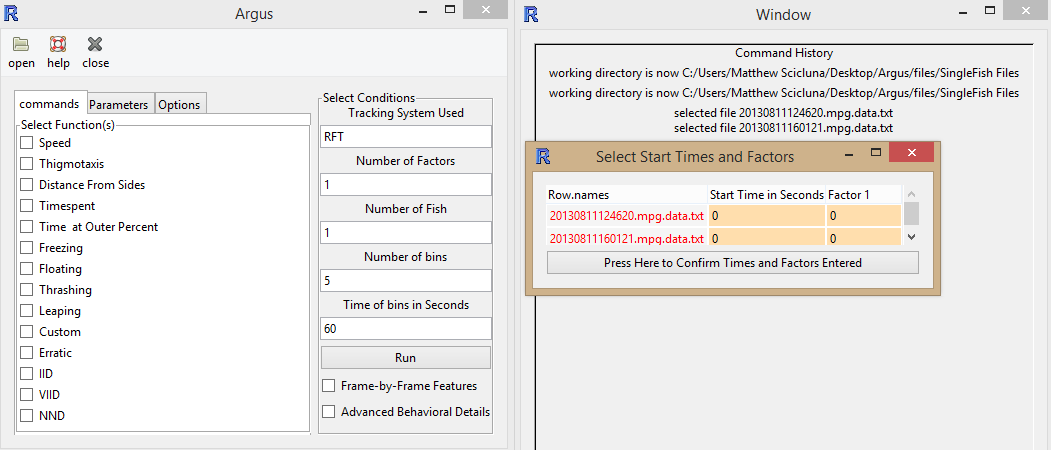
\includegraphics[width=120mm]{image18.png}
\caption{Selecting Categorical Variables and Cutoff Times}
\end{figure}

\pagebreak
\section{Navigating the Output File}
Figure 6.2 shows the output generated from the \texttt{Thrashing} function. Any other behavioral or trajectory variables will appear in different tabs in the output file, one behavior per tab. The leftmost column contains the file number for each trial, with each row being a trial. If the trials contain multiple fish being recorded, the variable values for each fish in each trial will be represented in cells below. The columns refer to each time bin for the trials. Each statistic is generated for each time bin you previously specified the amount and duration of. Because of this the trials all must have the same amount of bins, and if they do not columns with a dot will be generated as filler. This is done so the output file will be more SPSS friendly. Figures 6.3 and 6.4 show the detailed output file and the advanced output file, respectively. The detailed output file displays some additional information about the behavioral variables selected. The start times, end times, and total duration of each instance of a behavior recorded can be found in this output. The advanced output file contains frame-by-frame features for each fish with rows representing timepoints.
\paragraph{Frame-by-Frame Features}
Frame-by-frame features are  variables in themselves that describe the behavior of a fish at a specific point in time. These features can be used collectively to classify specific behaviors in machine learning algorithms. 

\begin{figure}[ht!]
\centering
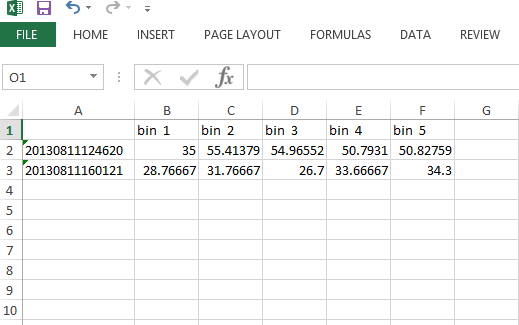
\includegraphics[width=130mm]{image15.png}
\caption{Regular Output From Argus}
\end{figure}
\pagebreak
\begin{figure}
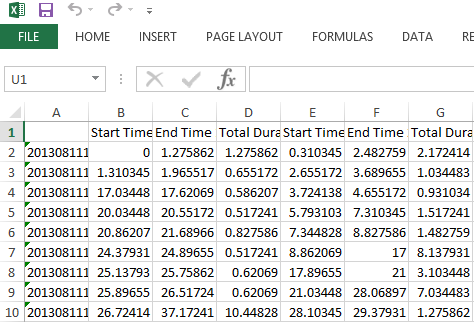
\includegraphics[width=130mm]{image16.png}
\caption{Detailed Behavioral Output From Argus}
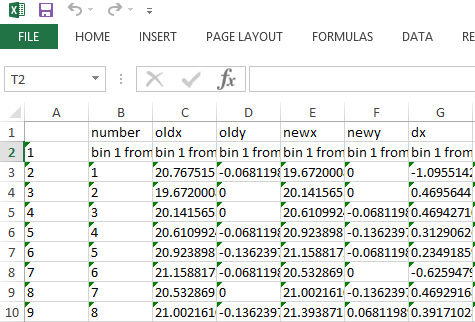
\includegraphics[width=130mm]{image17.png}
\caption{Advanced Output From Argus}
\label{overflow}
\end{figure}


\end{document}